\subsection{Performance Analysis}
\label{sec:evaluation-performance-analysis}
Let us now consider the experimental results about system performance recorded by our simulator.
In all the experiments we have considered values stated in Section~\ref{sec:performance-modeling-specification-model} with a preemption policy based on \textit{random selection}.

\subsection{Transient Analysis}
\label{sec:evaluation-transient-analysis}
First, we conduct a \textit{transient analysis} to evaluate the system stationary in order to (i) prove its convergence to the steady-state and (ii) estimate the duration of the transient period.
%
In fact, given a system that converges to stationary, the knowledge of the duration of the transient period is really important to conduct an effective performance evaluation. 
%
In particular, even if there exist techniques to reduce the impact of transitory measurements on the final insights, having an estimate for the duration of the transient period allows the analyst to focus performance evaluation on a system in its stationary conditions.

In Figures \ref{fig:evaluation-transient-analysis-throughput-1} and \ref{fig:evaluation-transient-analysis-throughput-2} we show the transient analysis for system running the Off-Loading Policy and 2, respectively. 
In this experiment we focused on the global system throughput as it can be considered a good representation of the dependency of the system to its initial state.
The experiment has been conducted considering an ensemble of $5$ replications, where the $i+1$-th replication is initialized with the last seed of the $i$-th replication, so as to achieve the best decoupling between random sequences of different replications.

The results show that the system reaches the steady-state in about $800$ simulated seconds, in both cases.
This result is not surprising because the presence of a stabilizing \textit{infinite-buffer centre}, i.e. the Cloud, largely compensates the possible instabilities produced by the \textit{finite-buffer centre}, i.e. the Cloudlet.

\begin{figure}
	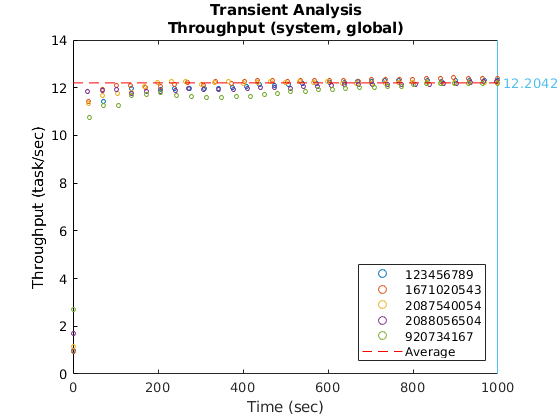
\includegraphics[width=\columnwidth]{fig/evaluation-transient-analysis-throughput}
	\caption{Transient analysis for the system with Off-Loading Policy 1.}
	\label{fig:evaluation-transient-analysis-throughput-1}
\end{figure}

\begin{figure}
	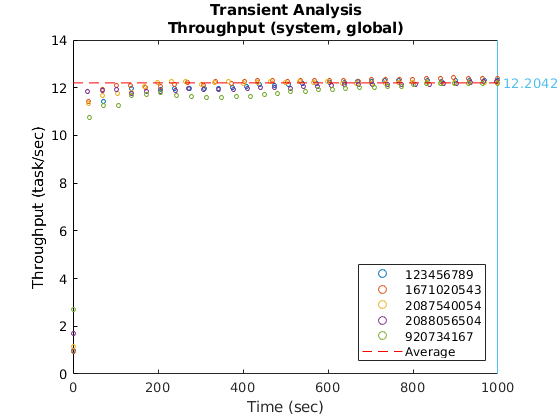
\includegraphics[width=\columnwidth]{fig/evaluation-transient-analysis-throughput}
	\caption{Transient analysis for the system with Off-Loading Policy 2.}
	\label{fig:evaluation-transient-analysis-throughput-2}
\end{figure}


\subsection{Steady-State Analysis}
Let us now focus on the performance evaluation in the steady-state, taking into account the following metrics:

\begin{enumerate}
	\item \textit{response time} both global and classed, both for the system as a whole and for each subsystem;
	
	\item \textit{throughput} both global and classed, both for the system as a whole and for each subsystem;
	
	\item \textit{population} both global and classed, both for the system as a whole and for each subsystem;
	
	\item \textit{interrupted ratio} for tasks belonging to the $2^{nd}$ class.
	
	\item \textit{interrupted response time} for tasks belonging to the $2^{nd}$ class.
\end{enumerate}

In our experiments we assumed the system with $S=N=20$ and batch means computations with $k=64$ batches of dimension $b=512$ each.
%
Theoretical results have been computed using the formulas presented in Section~\ref{sec:analytical-model}, assuming the experimentally computed values for routing probabilities shown in Table~\ref{tbl:evaluation-routing-probabilities} and $E[T_{clt,2,lost}]=1.47445;s.$.

In Tables \ref{tbl:evaluation-performance-metrics-1} and \ref{tbl:evaluation-performance-metrics-2}, we show the theoretical and experimental results for the system with Off-Loading Policy 1 and 2, respectively.

\begin{figure}
	\begin{center}
		\begin{tabular}{|c||c|c|}
			\hline
			Measure & Theoretical & Experimental\\
			\hline
			$a_{clt,1}$  & $0.978326334857105$ & $0.97911346521$ \\
			$a_{clt_2}$  & $0.603529764734761$ & $0.60502880468$ \\
			$r$          & $0.183573830264005$ & $0.15525744148$ \\	
			\hline
		\end{tabular}
	\end{center}
	\caption{Routing probabilities: comparison between the theoretical result, computed with the analytical model, and the experimental result, computed leveraging our simulator.}
	\label{tbl:evaluation-routing-probabilities}
\end{figure}

\begin{figure}
	\begin{center}
		\begin{tabular}{|c||c|c|}
			\hline
			Measure & Theoretical & Experimental\\
			\hline
			$E[N_{clt}]$  & $123456789$ & $123456789\pm 0.00342$ \\
			$E[N_{clt,1}]$  & $123456789$ & $123456789\pm 0.00342$ \\
			$E[N_{clt,2}]$  & $123456789$ & $123456789\pm 0.00342$ \\
			$E[T_{clt}]$  & $123456789$ & $123456789\pm 0.00342$ \\
			$E[T_{clt,1}]$  & $123456789$ & $123456789\pm 0.00342$ \\
			$E[T_{clt,2}]$  & $123456789$ & $123456789\pm 0.00342$ \\
			$X_{clt}$  & $123456789$ & $123456789\pm 0.00342$ \\
			$X_{clt,1}$  & $123456789$ & $123456789\pm 0.00342$ \\
			$X_{clt,2}$  & $123456789$ & $123456789\pm 0.00342$ \\
			\hline
			$E[N_{cld}]$  & $123456789$ & $123456789\pm 0.00342$ \\
			$E[N_{cld,1}]$  & $123456789$ & $123456789\pm 0.00342$ \\
			$E[N_{cld,2}]$  & $123456789$ & $123456789\pm 0.00342$ \\
			$E[T_{cld}]$  & $123456789$ & $123456789\pm 0.00342$ \\
			$E[T_{cld,1}]$  & $123456789$ & $123456789\pm 0.00342$ \\
			$E[T_{cld,2}]$  & $123456789$ & $123456789\pm 0.00342$ \\
			$X_{cld}$  & $123456789$ & $123456789\pm 0.00342$ \\
			$X_{cld,1}$  & $123456789$ & $123456789\pm 0.00342$ \\
			$X_{cld,2}$  & $123456789$ & $123456789\pm 0.00342$ \\
			\hline
			$E[N_{sys}]$  & $123456789$ & $123456789\pm 0.00342$ \\
			$E[N_{sys,1}]$  & $123456789$ & $123456789\pm 0.00342$ \\
			$E[N_{sys,2}]$  & $123456789$ & $123456789\pm 0.00342$ \\
			$E[T_{sys}]$  & $123456789$ & $123456789\pm 0.00342$ \\
			$E[T_{sys,1}]$  & $123456789$ & $123456789\pm 0.00342$ \\
			$E[T_{sys,2}]$  & $123456789$ & $123456789\pm 0.00342$ \\
			$X_{sys}$  & $123456789$ & $123456789\pm 0.00342$ \\
			$X_{sys,1}$  & $123456789$ & $123456789\pm 0.00342$ \\
			$X_{sys,2}$  & $123456789$ & $123456789\pm 0.00342$ \\
			\hline
			$E[T_{restarted}]$  & $123456789$ & $123456789\pm 0.00342$ \\
			$RestartRatio$  & $123456789$ & $123456789\pm 0.00342$ \\			
			\hline
		\end{tabular}
	\end{center}
	\caption{Performance metrics for the system with Off-Loading Policy 1.}
	\label{tbl:evaluation-performance-metrics-1}
\end{figure}

\begin{figure}
	\begin{center}
		\begin{tabular}{|c||c|c|}
			\hline
			Measure & Theoretical & Experimental\\
			\hline
			$E[N_{clt}]$  & $123456789$ & $123456789\pm 0.00342$ \\
			$E[N_{clt,1}]$  & $123456789$ & $123456789\pm 0.00342$ \\
			$E[N_{clt,2}]$  & $123456789$ & $123456789\pm 0.00342$ \\
			$E[T_{clt}]$  & $123456789$ & $123456789\pm 0.00342$ \\
			$E[T_{clt,1}]$  & $123456789$ & $123456789\pm 0.00342$ \\
			$E[T_{clt,2}]$  & $123456789$ & $123456789\pm 0.00342$ \\
			$X_{clt}$  & $123456789$ & $123456789\pm 0.00342$ \\
			$X_{clt,1}$  & $123456789$ & $123456789\pm 0.00342$ \\
			$X_{clt,2}$  & $123456789$ & $123456789\pm 0.00342$ \\
			\hline
			$E[N_{cld}]$  & $123456789$ & $123456789\pm 0.00342$ \\
			$E[N_{cld,1}]$  & $123456789$ & $123456789\pm 0.00342$ \\
			$E[N_{cld,2}]$  & $123456789$ & $123456789\pm 0.00342$ \\
			$E[T_{cld}]$  & $123456789$ & $123456789\pm 0.00342$ \\
			$E[T_{cld,1}]$  & $123456789$ & $123456789\pm 0.00342$ \\
			$E[T_{cld,2}]$  & $123456789$ & $123456789\pm 0.00342$ \\
			$X_{cld}$  & $123456789$ & $123456789\pm 0.00342$ \\
			$X_{cld,1}$  & $123456789$ & $123456789\pm 0.00342$ \\
			$X_{cld,2}$  & $123456789$ & $123456789\pm 0.00342$ \\
			\hline
			$E[N_{sys}]$  & $123456789$ & $123456789\pm 0.00342$ \\
			$E[N_{sys,1}]$  & $123456789$ & $123456789\pm 0.00342$ \\
			$E[N_{sys,2}]$  & $123456789$ & $123456789\pm 0.00342$ \\
			$E[T_{sys}]$  & $123456789$ & $123456789\pm 0.00342$ \\
			$E[T_{sys,1}]$  & $123456789$ & $123456789\pm 0.00342$ \\
			$E[T_{sys,2}]$  & $123456789$ & $123456789\pm 0.00342$ \\
			$X_{sys}$  & $123456789$ & $123456789\pm 0.00342$ \\
			$X_{sys,1}$  & $123456789$ & $123456789\pm 0.00342$ \\
			$X_{sys,2}$  & $123456789$ & $123456789\pm 0.00342$ \\
			\hline
			$E[T_{restarted}]$  & $123456789$ & $123456789\pm 0.00342$ \\
			$RestartRatio$  & $123456789$ & $123456789\pm 0.00342$ \\			
			\hline
		\end{tabular}
	\end{center}
	\caption{Performance metrics for the system with Off-Loading Policy 2.}
	\label{tbl:evaluation-performance-metrics-2}
\end{figure}

%%
% DISTRIBUTION ANALYSIS
%%
%\subsection{Distribution Analysis}
%\label{sec:evaluation-distribution-analysis}
%In this Section we show the distribution analysis of the Cloudlet global throughput. 
%In particular, we focus on both (i) the Probability Density Function (PDF) estimation leveraging distribution fitting, and (ii) the comparison between theoretical and experimental Cumulative Distribution Function (CDF).

%In Figure~\ref{fig:evaluation-distribution-analysis-pdf-throughput-cloudlet-global} and  Figure~\ref{fig:evaluation-distribution-analysis-cdf-throughput-cloudlet-global} we show the PDF estimation and the CDF analysis, respectively, for the global Cloudlet throughput when $S=N=20$, where we adopted the \textit{Freedman-Diaconis Rule} for the binning schema.
%Results show that the best fitting is the \textit{Normal Distribution} with parameters $\mu\approx7.403$ and $\sigma\approx0.364$.
%
%The Normal behavior shown here can be considered as a further good proof of both the system stationary and the effectiveness of the batch means as a tool to study steady-state statistics.

%\begin{figure}
%	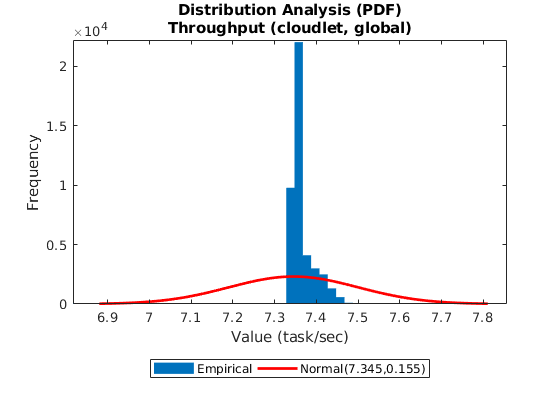
\includegraphics[width=\columnwidth]{fig/evaluation-distribution-analysis-pdf-throughput-cloudlet-global}
%	\caption{Distribution analysis (Probability Distribution Function)for the Cloudlet global throughput with threshold $S=N=20$.}
%	\label{fig:evaluation-distribution-analysis-pdf-throughput-cloudlet-global}
%\end{figure}

%\begin{figure}
%	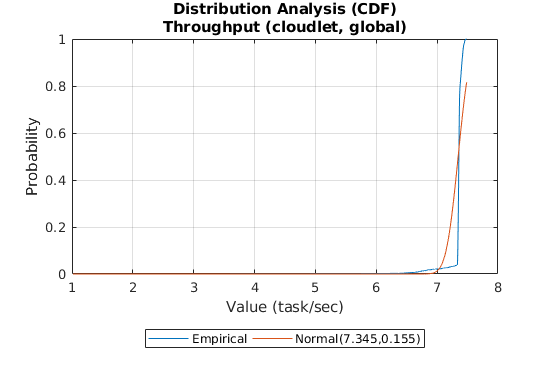
\includegraphics[width=\columnwidth]{fig/evaluation-distribution-analysis-cdf-throughput-cloudlet-global}
%	\caption{Distribution analysis (Cumulative Distribution Function) for the Cloudlet global throughput with threshold $S=N=20$.}
%	\label{fig:evaluation-distribution-analysis-cdf-throughput-cloudlet-global}
%\end{figure}